\section{Исследование ряда}
\subsection{Исследование сходимости ряда}

Пусть задана функция
\begin{equation} 
u(x) = \sum_{k=0}^{+\infty}{\hat{u}_k P_k(x)}, \;x \in [-1;1],
\end{equation}
определено пространство $$L_2[-1,1] = \left\lbrace  u \big| \norm{u}<\infty \right\rbrace,$$
\begin{explanationx}
\item[где] $\norm{u} = \sqrt{(u,u)},\; (u,v) = \int_{-1}^{1}{u(x)v(x)\dd{x}}.$
\end{explanationx}

Пусть также определены частичные суммы 
\begin{equation}
 u_N(x) = \sum_{k=0}^{N}{\hat{u}_k P_k(x)}, \;x \in [-1;1],\;N\in \mathbb{N}.
\end{equation}
Тогда, согласно~\cite{Legendre08AMS} (восходящей к  ~\cite{ApproxSob82AMS}), если $u \in H^{2q}[-1,1]$, то для $q\geqslant0$ 
\begin{equation}
\sqrt{\sum_{k=N+1}^{+\infty}{\norm{P_k}^2{\hat{u}_k}^2}} = \norm{u-u_N} \leqslant CN^{-2q}\norm{u}_{H^{2q}[-1,1]},
\end{equation}
\begin{explanationx}
\item[где] $H^p[-1,1]$ ---  пространство Соболева:
$$ H^p[-1,1]=\left\lbrace u\in\L^2[-1,1] \big| \norm{u}_{H^{p}[-1,1]}^2 = \sum_{k=0}^{p}\norm{u^{(k)}}^2 < \infty \right\rbrace ;$$
\item  $C$  --- некоторая константа, согласно~\cite[Th. 2.1]{ApproxSob82AMS} равная $2^{-d/2+1}$ ($d$ --- размерность $x$, в~\cite{Legendre08AMS} $d=1$).
\end{explanationx}

Исходя из этого, если сама $u$ имеет конечную норму, и если нормы ее производных по $x$ вплоть до $p$-го порядка ($p>0$) --- конечны, то ряд сходится в $L_2$.

В нашем случае, при ограниченном максимуме
   \begin{equation}
	\max_{n \in \mathbb{N}} \abs{\int_{-1}^{1}{f(\theta)P_n (\cos	\theta) \dd{\cos\theta}}} < \infty
   \end{equation}
   норма $\norm{u}$ тоже ограничена, т.к. сходится ряд $ \sum_{k=1}^{+\infty}{k^{-2}}$.
   Можно показать, что сумма норм ее производных также конечна. Однако, основная задача --- проверка сходимости в $L_1$. Оценим остаток ряда, используя явное выражение функции $f$.     

    \subsection{Определение остатка ряда}
Вспомним полученное выражение для функции $u(t,\theta)$:
\begin{equation}
	\label{eq: u_research}
   	 \begin{split}
   	 u(\theta,t) 
	 =& \beta \frac{R^2}{K}\sum_{k=1}^{+\infty}{
	   		 \frac{(4k+1)P_{2k-2}(0)}{16k^2 (2k+1)(k+1)}\left(1 - e^{-2k(1+2k)\frac{K}{cR^2} t}
		 \right)P_{2k}(\cos\theta)} + \\
	 &+ \frac{\beta}{4c} t + \beta \frac{R^2}{4K}
	   		 \left(1 - e^{-2\frac{K}{cR^2} t}
		 \right)\cos\theta.
   	  \end{split} 
\end{equation}
   	 
Пусть для всех $n \in \mathbb{N}$
\begin{equation}
	\label{eq: I}
	I_n = \sum_{k=n}^{+\infty}{\frac{4k+1}{16k^2 (2k+1)(k+1)}}
\end{equation}
и 
\begin{equation}
	\label{eq: G}
	G_n = \beta \frac{R^2}{K}\sum_{k=1}^{+\infty}{
	   		 \frac{(4k+1)P_{2k-2}(0)}{16k^2 (2k+1)(k+1)}\left(1 - e^{-2k(1+2k)\frac{K}{cR^2} t}
		 \right)P_{2k}(\cos\theta)}. 
\end{equation}
Заметим, что $\abs{G_{n}}$ является оценкой $n$-го остатка ряда~(\ref{eq: u_research}), точнее --- погрешность метода в вычислениях функции $u$ при использовании $n$ членов ряда~(\ref{eq: u_research}) не превосходит по модулю $\abs{G_{n}}$.

Функции $\{P_n(\cos\theta)\}$ являются ограниченными на множестве~$[-1;1]$ (см.~\cite[часть~II, \S\,1 п.\,7]{TihonovAndSamarskiy99EMF}):
   	 \begin{equation}
   	 \label{eq: research_abs_P_n}
   	 \abs{P_n(x)} \leqslant 1, \qquad \forall n \in \mathbb{N}_0.
   	 \end{equation} 
Учитывая это, а также то, что для всех $k \in \mathbb{N}$ $e^{-2k(1+2k)\frac{K}{cR^2} t} \leqslant 1$, получаем оценки для $\{G_n\}$:
\begin{equation}
	\label{eq: G_and_I}
	G_n \leqslant \beta \frac{R^2}{K}I_n \cdot 1 \cdot 1 = \beta \frac{R^2}{K}I_n, \qquad \forall n \in \mathbb{N}. 
\end{equation}

 Оценим сумму $I_n$:
	\begin{equation}
	\label{eq: I<frac_1_8k^3}
	 \begin{split}
		I_n &<\sum_{k=n}^{+\infty}{\frac{4k+2}{16k^2 (2k+1)(k+1)}} \\
		 &=\sum_{k=n}^{+\infty}{\frac{1}{8k^2 (k+1)}} \\
		 &<\sum_{k=n}^{+\infty}{\frac{1}{8k^3}}. \\
     \end{split}
	\end{equation}
	
	Рассмотрим функцию $h(\xi)=\rfrac{1}{8}\xi^{-3}$ и последовательность $w_n=\rfrac{1}{8}n^{-3}$. Очевидно, что $h(\xi)$ определена на интервале $[1;+\infty)$, и, кроме того, убывает на нем. Заметим также, что
	\begin{equation}
w_{k+1} \leqslant h(\xi) \leqslant w_k, \qquad k \in \mathbb{N},\; k\leqslant x \leqslant k+1.
	\end{equation}
	
	Поэтому справедливы следующие неравества (см. \cite[стр. 347]{matanMSU}):
	\begin{equation}
	w_{k+1} \leqslant \int_{k}^{k+1}h(\xi)\dd{\xi} \leqslant w_k, \qquad k \in \mathbb{N},\; k\leqslant x \leqslant k+1.
	\end{equation}
	
	Суммируя по $k$ от $n_0\in \mathbb{N}$ до бесконечности, получаем:
	\begin{equation}
	\label{eq: sum_w_k+1}
	\sum_{k=n_0}^{+\infty}{w_{k+1}} \leqslant \sum_{k=n_0}^{+\infty}\int_{k}^{k+1}h(\xi)\dd{\xi} = \int_{n_0}^{+\infty}{h(\xi)\dd{\xi}}.
	\end{equation}
	
	Вычислим теперь интеграл $\int_{n_0}^{+\infty}{h(\xi)\dd{\xi}}$:
	\begin{equation}
	\label{eq: int_h(xi)<frac_1_16_n_0^-2}
	\int_{n_0}^{+\infty}{h(\xi)\dd{\xi}} = \frac{1}{8}\int_{n_0}^{+\infty}{\xi^{-3}\dd{\xi}} = \frac{1}{8}\left( 0 - ( - \frac{1}{2} n_0^{-2}) \right) = \frac{1}{16}n_0^{-2}.
	\end{equation}
	Таким образом, из формул~(\ref{eq: I<frac_1_8k^3}), (\ref{eq: sum_w_k+1}) и~(\ref{eq: int_h(xi)<frac_1_16_n_0^-2}) мы можем оценить $I_{n_0}$:
	\begin{equation}
	\label{eq: I_n_accuracy}
	I_{n_0} < \frac{1}{16}n_0^{-2}, \qquad n_0 \in \mathbb{N}.
	\end{equation}
	
	Наконец, из системы~(\ref{eq: G_and_I}) получаем, что 
	\begin{equation}
	\label{eq: G_n_accuracy}
		G_{n_0} < \frac{\beta R^2}{16K} n_0^{-2}, \qquad n_0 \in \mathbb{N}.
	\end{equation}
	
	Учитывая пояснения к формуле~(\ref{eq: G}), получаем, что для достижения точности $\varepsilon$ вычисления функции $u$ достаточно использовать 
	$$n_0 = \Bigg\lceil \sqrt{\frac{\beta R^2}{16K\varepsilon}}\Bigg\rceil$$ членов ряда~(\ref{eq: u_research}).
		
	\section{Написание программы}
	\subsection{Описание использованных языков, приложений и пакетов}
	Для написания программы были использованы языки \textit{Java} и \textit{Scala}. Код на языке Scala 2.11 был написан в среде \textit{Scala IDE build of Eclipse SDK}, версия IDE --- 4.1.0. Графический интерфейс был написан в среде \textit{NetBeans 8.02} на языке Java 8. Итоговая версия была собрана с использованием \textit{IntelliJ IDEA 15.0}. 

	При написании интерфейса были использованы пакеты \textit{jfreechart-1.0.19}, \textit{jcommon-1.0.23} и \textit{jfreesvg-2.0}.

	Программа может быть запущена на компьютерах с установленным \textit{JDK 8}. 
	
	\subsection{Описание кода}
	\subsubsection{}
	Объект для описания исходных данных представлен на следующем листинге. 
	\lstinputlisting[language=scala, mathescape, numbers=left]{/home/misha/latex/EMF/Data.scala}		
	
	Процедура \textit{init} выполняет инициализацию множества полиномов Лежандра в точке $0$, и вызывается лишь один раз за все время работы программы. 
	\subsubsection{} 
	Основные вычисления (в частности, вычисление искомой функции $u$) реализованы в объекте Solution. Сложные функции пояснены комментариями. 
	\lstinputlisting[language=scala, mathescape, numbers=left]{/home/misha/latex/EMF/Solution.scala}	
	
	Класс, отвечающий за интерфейс программы, является громоздким (в нем 352 строки), к тому же, он не является обязательным для выполнения основной задачи --- вычисления функции $u$.  
	
	Полную версию программы можно посмотреть по адресу~\url{https://github.com/Mikhail42/EMPh}. 	
	
	\subsection{Тестирование}
	Тестирование происходило в операционной системе \textit{Ubuntu 15.10}. 
	Примеры результатов выполнения программы представлены ниже. 
	\begin{figure}[h]
	\begin{center}
		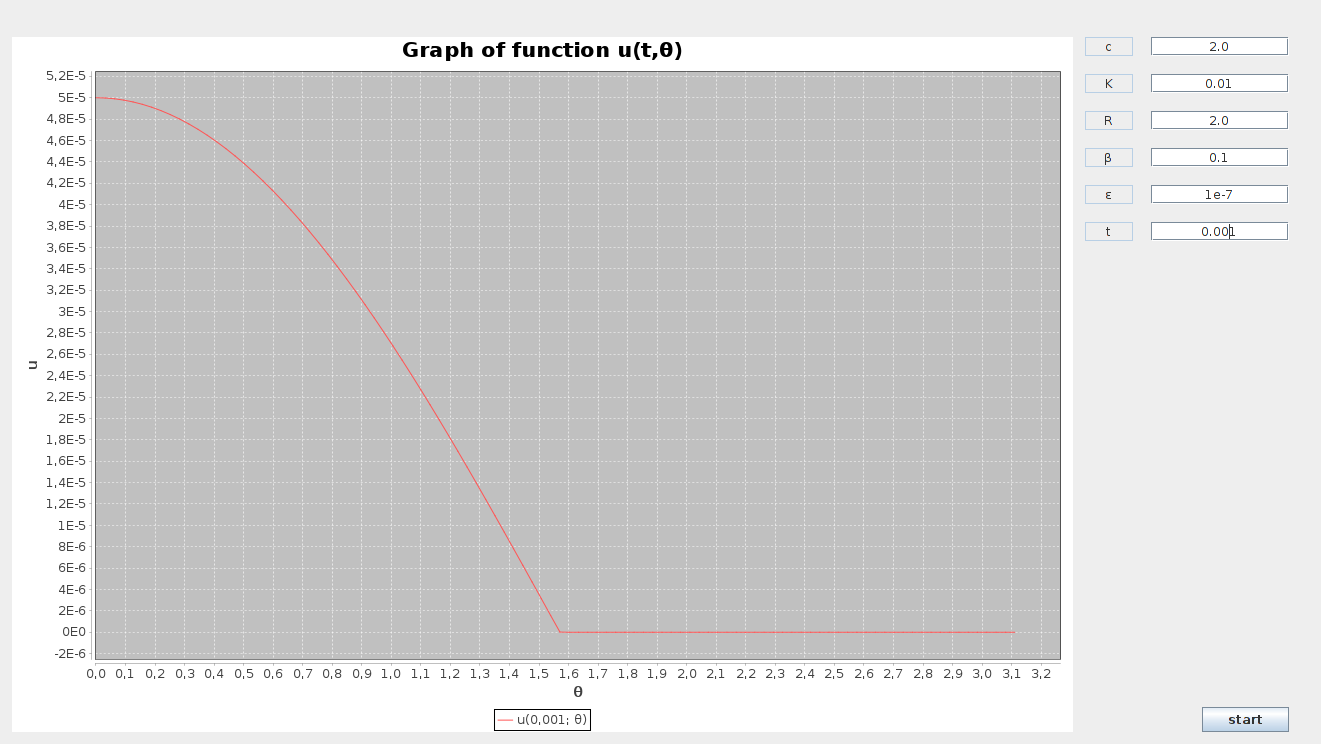
\includegraphics[width=1\linewidth]{screen_t0p001.png}
		\caption{График с исходными значениями при $t=0.001$}
		\label{fig: screen_t0p001}
	\end{center}
	\end{figure}
	\begin{figure}[h]
	\begin{center}
		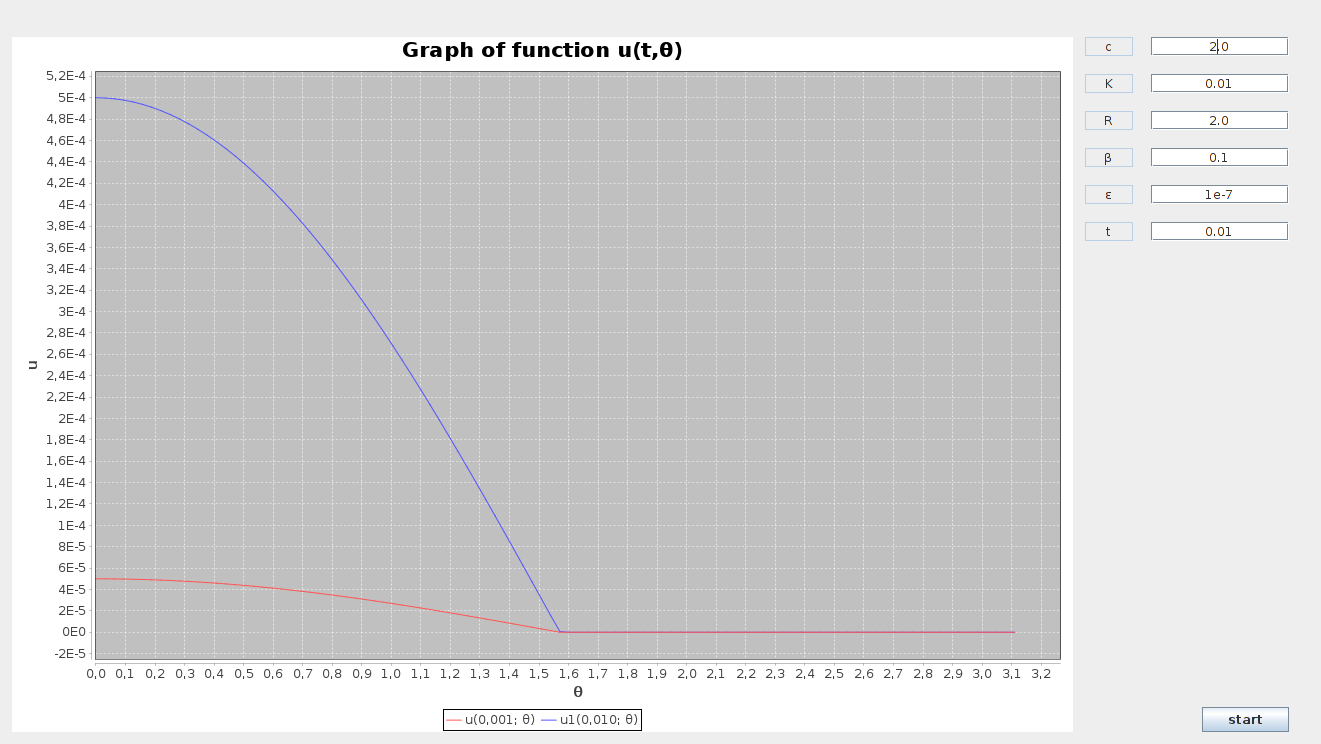
\includegraphics[width=1\linewidth]{screen_t0p01.png}
		\caption{График после изменения $t$ на $0.01$}
		\label{fig: screen_t0p001}
	\end{center}
	\end{figure}
	\begin{figure}[h]
	\begin{center}
		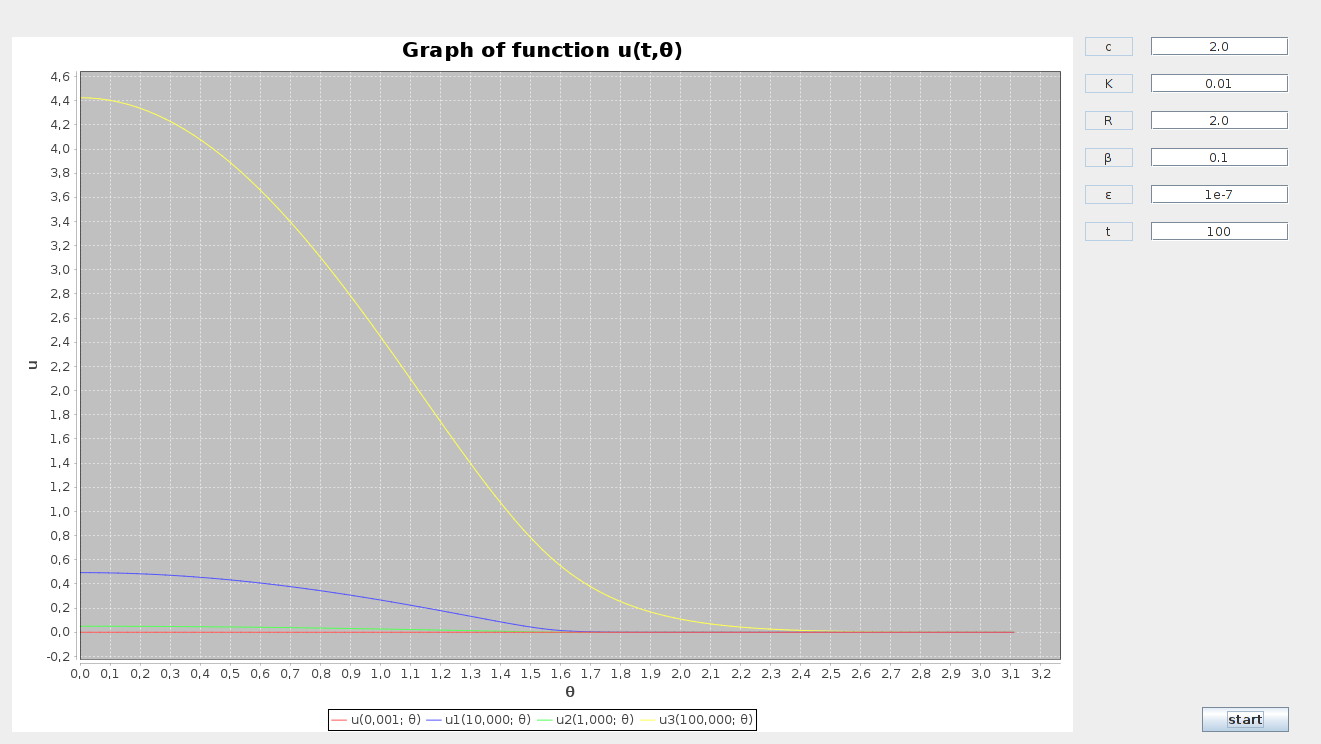
\includegraphics[width=1\linewidth]{screen_dif_t.png}
		\caption{Графики при различных $t\geqslant 0.001$}
		\label{fig: screen_t0p001}
	\end{center}
	
	\end{figure}
	\begin{figure}[h]
	\begin{center}
		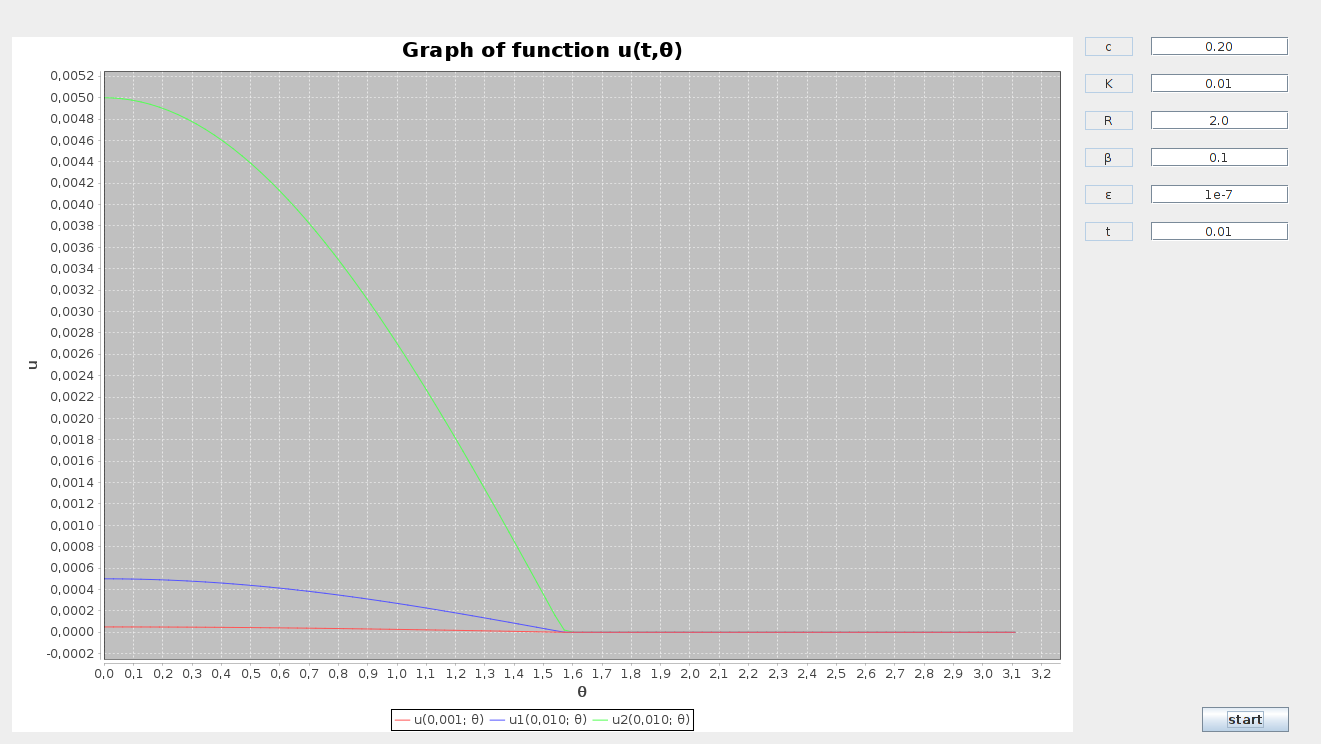
\includegraphics[width=1\linewidth]{screen_c0p2.png}
		\caption{График после изменения $c$ на $0.2$}
		\label{fig: screen_t0p001}
	\end{center}
	\end{figure}